\chapter{Psychophysiological Interactions (PPI)}

\section{Theoretical background}

Psychophysiologic interactions (PPI) model the response in one cortical area as the influence of another region and its interaction with an experimental treatment (sensory stimulus, task, etc.) \cite{ppi}. This technique is one way of examining effective connectivity, or the influence that one neural system exerts on another \cite{func1}. Mechanistically, a PPI analysis involves the following steps. 
\begin{enumerate}
\item Performing a standard GLM analysis.
\item Extracting BOLD signal from a source region identified in the GLM analysis.
\item Forming the interaction term (source signal x experimental treatment)
\item Performing a second GLM analysis that includes the interaction term, the source region's extracted signal and the experimental vector in the design. The inclusion of the source region's signal and the experimental vector is analogous to including the main effects in an ANOVA in order to make an inference on the interaction.
\end{enumerate} 

Forming the proper interaction term turns out to be a challenge because of the unique characteristics of fMRI (BOLD) data in which the underlying neural signal is convolved with a hemodynamic response function. However, interactions in the brain take place at the neural and not the hemodynamic level. Therefore, appropriate models of the interactions require the neural signal, which is not measured directly, but instead must be derived by deconvolving the HRF. The PPI software (\texttt{spm\_peb\_ppi.m}) was developed in order to provide robust deconvolution of the HRF and the proper derivation of the interaction term \cite{gitelman_03}.

\section{Practical example}

The dataset in this exercise is from one subject who was studied in the \cite{buchel1998} report and refers to the ``attention to motion'' dataset available from the SPM website\footnote{\url{http://www.fil.ion.ucl.ac.uk/spm/data/attention/}}. It has already been described in the previous chapter for DCM.

The goal is to use PPI to examine the change effective connectivity between V2 and V5 while the subject observes visual motion (radially moving dots) under the experimental treatments of attending vs. not attending to the speed of the dots. The psychophysiologic interaction can be conceived of as looking for a significant difference in the regression slopes of V1 vs. V5 activity under the influence of the different attentional states \cite{ppi}.

\subsection{GLM analysis - Design setup and estimation}

This dataset has already been preprocessed (coregistered, normalised and smoothed) using an earlier version of SPM.

\begin{enumerate}
\item The analysis directory should include
\begin{enumerate}
\item A directory named \texttt{functional}, which includes the preprocessed fMRI volumes.
\item A directory named \texttt{structural}, which includes a T1 structural volume
\item Files: \texttt{factors.mat}, \texttt{block\_regressors.mat}, \texttt{multi\_condition.mat} and \texttt{multi\_block\_regressors.mat}.
\item You will also need to make 2 empty directories called \texttt{GLM} and \texttt{PPI} for performing the analyses.
\end{enumerate}

\item In \matlab\ type
\begin{verbatim}
>> cd 'path-to-analysis-directory'
>> spm fmri
\end{verbatim}
\item From the Tasks menu at the top of the Graphics window select \textsc{Batch}
\item Select \textsc{New ``Stats''} from the Options box, Figure 1.1.

\begin{figure}[!ht]
\centering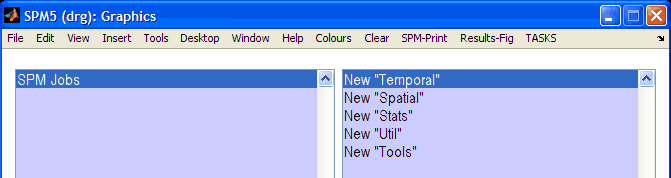
\epsfig{file=ppi/select-stats,width=85mm}
\caption{\em Select \textsc{New ``Stats''} from the Options box}
\label{ppi_fig1}
\end{figure}

\item Click \textsc{Stats} in the Batch box and then select \textsc{New ``Fmri model specification''}, \textsc{New ``Model Estimation''} and \textsc{``New Contrast Manager''} from the Options box, Figure 1.2.

\begin{figure}[ht]
\centering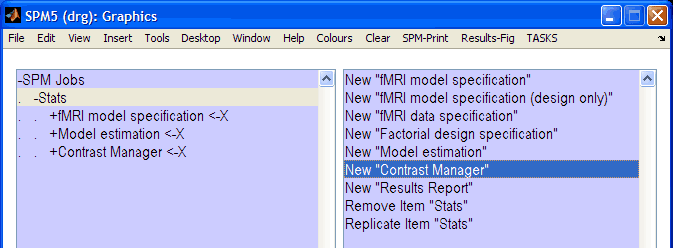
\epsfig{file=ppi/select-batch-components,width=100mm}
\caption{\em Click \textsc{Stats} in the Batch box and then select \textsc{New ``Fmri model specification''}, \textsc{New ``Model Estimation''} and \textsc{``New Contrast Manager''} from the Options box}
\label{ppi_fig2}
\end{figure}

\item Right click in the Batch box then choose \textsc{Exp/Con All > Expand All}, Figure 1.3\\\\

\begin{figure}[!ht]
\centering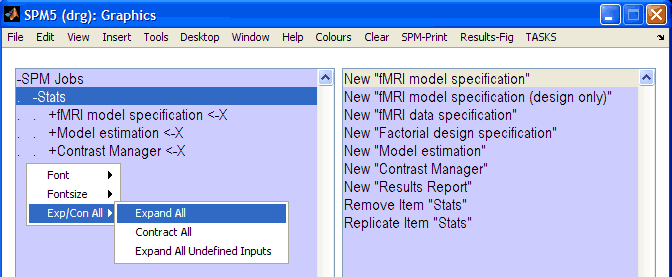
\epsfig{file=ppi/expand-batch-components,width=85mm}
\caption{ \em{Right click the Batch box then choose \textsc{Exp/Con All > Expand All}}}
\label{ppi_fig3}
\end{figure}

\textbf{Fill in the \textsc{Fmri model specification}} (Figure 1.4)

\begin{figure}[!ht]
\centering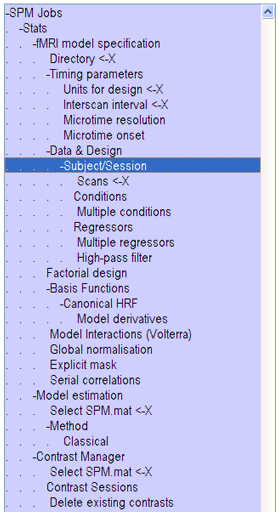
\epsfig{file=ppi/expanded-batch-newsubj,width=75mm}
\caption{\em Click \textsc{Data \& Design} and Choose \textsc{New "Subject/Session"}}
\label{ppi_fig4}
\end{figure}

%\begin{figure}[!ht]
%\centering\epsfig{file=ppi/expanded-batch,width=75mm}
%\caption{\em Fill in the \textsc{Fmri model specification}}
%\label{ppi_fig4}
%\end{figure}

\item Click \textsc{Directory} and choose the \texttt{GLM} directory that you made above.
\item \textsc{Units for design} [\textsc{scans}]
\item \textsc{Interscan interval} [3.22]
\item \textsc{Microtime resolution} [16]
\item \textsc{Microtime onset} [1]
\item Click \textsc{Data \& Design}, Choose \textsc{New "Subject/Session"} from the options box then right click the Batch box and expand all, Figure 1.4.
\item Click \textsc{Scans} and choose all the functional scans \texttt{snffM00587\_00xx.img}. There should be 360 \texttt{*.img} files.
\item The experimental conditions can be defined either individually or using a multiple condition \texttt{mat}-file. This exercise shows both methods for educational purposes. When doing an actual analysis you can just follow one of the two approaches below.\\\\\\
\textbf{Define conditions individually}\\
\item Load the mat file containing the individual conditions:
\begin{verbatim}
>> load factors.mat
\end{verbatim}
You can look at the loaded variables by typing the variable names.
( \texttt{stat} = stationary, \texttt{natt} = no attention, \texttt{att} = attention)
\begin{verbatim}
>> stat
>> natt
>> att
\end{verbatim}
\item Click \textsc{Conditions} under \textsc{Subject/Session} and from the Options box add 3 \textsc{``New Conditions''}, then expand all.

\item Condition 1: Name = \texttt{Stationary}, \textsc{Onsets} = \texttt{stat}, \textsc{Durations} = 10
\item Condition 2: Name = \texttt{No-attention}, \textsc{Onsets} = \texttt{natt}, \textsc{Durations} = 10
\item Condition 3: Name = \texttt{Attention}, \textsc{Onsets} = \texttt{att}, \textsc{Durations} = 10
\item Next you will enter 3 regressors to model block effects. This will account for the fact that the experiment took place over 4 runs that have been concatenated into a single session to make the PPI analysis easier. First load the regressors:
\begin{verbatim}
>> load block_regressor.mat
\end{verbatim}
\item Click \textsc{Regressors} and add 3 \textsc{New Regressors}, then expand all.
\item Regressor 1: \textsc{Name} = \texttt{Block 1}, \textsc{Value} = \texttt{block1}
\item Regressor 2: \textsc{Name} = \texttt{Block 2}, \textsc{Value} = \texttt{block2}
\item Regressor 3: \textsc{Name} = \texttt{Block 3}, \textsc{Value} = \texttt{block3}\\\\

\textbf{Define conditions using multiple condition and multiple regressor files}\\
\item If you would like to look at the organization of the variables in the multiple condition file, first load it.
\begin{verbatim}
>> load multi_condition.mat
>> names
>> onsets
>> durations
\end{verbatim}
Notice that there are three variables organized as cell arrays. The variables in a multiple condition file must always be named: 'names', 'onsets', and 'durations'
\textit{(Note: You only need to do this step if you want to look at the organization of the variables. In contrast to defining conditions individually, as shown above, when using a multiple condition file you do not have to load the file in order to enter it into the design.)}\\
\item To use the multiple conditions file in the design, click \textsc{Multiple Conditions}, then \textsc{Specify Files} in the Options box and choose the \texttt{multi\_condition.mat} file.
\item Next you will enter the 3 regressors to model block effects by using a multiple regressor file. To look at the organization of the multiple regressor variable, first load it. \textit{(Again you do not have to load the multiple regressor file in order to use it. This step is just to allow you to examine the variable.)}
\begin{verbatim}
>> load multi_block_regressor.mat
>> R
\end{verbatim}
Notice that this file contains a single variable, \texttt{R}, which has each regressor in a separate column.
\item To use the multiple regressor file, click \textsc{Multiple Regressor} then select the  \texttt{multi\_block\_regressor.mat} file\\\\

\textbf{Complete the design setup}\\
\item \textsc{High-pass filter} [192] (Note: most designs will use a high-pass filter value of 128. However, this dataset requires a longer high-pass filter in order not to lose the low frequency components of the design.)
\item \textsc{Factorial design} is not used
\item The \textsc{Basis function} is the \textsc{canonical HRF} as shown and \textsc{Model derivatives} [\textsc{No derivatives}]
\item \textsc{Model Interactions (Volterra)}: [\textsc{Do not model interactions}]
\item \textsc{Global normalisation} [\textsc{None}]
\item \textsc{Explicit mask} [\textsc{None}]
\item \textsc{Serial correlations} [\textsc{AR(1)}]
\item Under \textsc{Model estimation} click \textsc{Select \texttt{SPM.mat}} then choose \textsc{Output from ``fMRI model specification''} from the Options box.
\item Under \textsc{Contrast Manager} click \textsc{Select \texttt{SPM.mat}} then choose \textsc{Output from ``Model estimation''} from the Options box.
\item Click \textsc{Contrast Sessions} then click \textsc{New ``F-contrast''} once, and \textsc{New ``T-contrast''} twice from the Options box, and Expand all.
\item Click \textsc{F-contrast} $\rightarrow$ \textsc{Contrast vectors} and then choose \textsc{New ``F contrast vector''} 3 times from the Options box
\item Under the F-contrast the name is: \texttt{Effects of Interest}
\item The F contrast vectors are as follows.
Enter each one in turn into an F contrast vector.
\begin{verbatim}
1 0 0 0 0 0 0
0 1 0 0 0 0 0
0 0 1 0 0 0 0
\end{verbatim}
\item For the first T-contrast click \textsc{Name}, then click \textsc{Specify Text} in the Options box and enter: \texttt{Attention}.
\item Click \textsc{T contrast vector}, then \textsc{Specify Text} in the Options box and enter: \texttt{~0~-1~1~0~0~0~0} (Note the order of the conditions in the design matrix is: Stationary, NoAttMot and AttMot).
\item For the second T-contrast the name is: \texttt{Motion}. The vector is: \texttt{-2~1~1~0~0~0~0}
\item Click the \textsc{Save} button and save the batch file.\\

\textbf{Design estimation}\\
\item If everything has been entered correctly the \textsc{Run} button is no longer grayed out. Click \textsc{Run} to estimate the design.
\item The design matrix should look as shown in Figure 1.5, below.

\begin{figure}[!ht]
\centering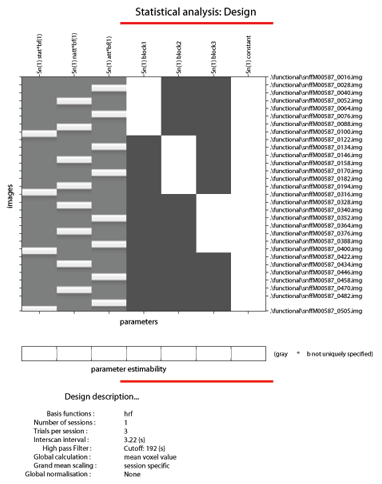
\epsfig{file=ppi/glm-design-matrix,width=85mm}
\caption{\em Design matrix}
\label{ppi_fig5}
\end{figure}
\end{enumerate}

\subsection{GLM analysis - Results}

\begin{enumerate}
\item Click \textsc{Results} and select the \texttt{SPM.mat} file.
\item Choose the \texttt{Attention} contrast
\item Mask with other contrasts [No]
\item Title for comparison [Attention]
\item p value adjustment to control [None]
\item threshold {T or p value} [0.0001]
\item \& extent threshold {voxels} [10]
\item You should see an SPM that looks like the one shown below, Figure 1.6. Note the Superior Parietal and Dorso-Lateral Prefrontal activations, among others. By selecting \textsc{overlays} $\rightarrow$ \textsc{sections}, and selecting the normalised structural image, you should be able to identify the anatomy more accurately.

\begin{figure}[!ht]
\centering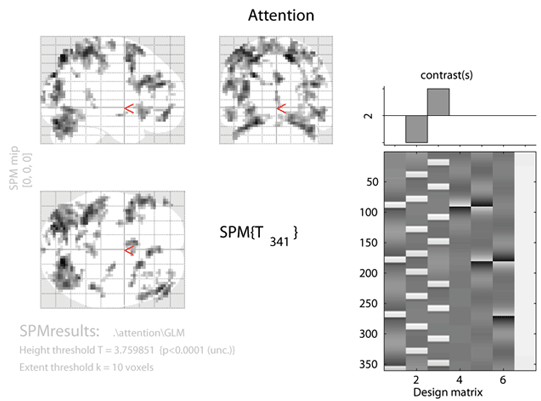
\epsfig{file=ppi/attention-contrast,width=85mm}
\caption{\em Statistical parametric map for the \texttt{Attention} contrast}
\label{ppi_fig6}
\end{figure}

\item To look at the \texttt{Motion} contrast where \texttt{Attention} is greater than \texttt{No Attention}, click \textsc{Results}, choose the \texttt{SPM.mat} file and choose the \texttt{Motion} contrast.
\item Mask with other contrasts [Yes]
\item Select contrast for masking: Choose the \texttt{Attention} contrast
\item Uncorrected mask p-value [0.01]
\item Nature of Mask: [inclusive]
\item Title for comparison: leave as the defaults, which is [Motion  (masked [incl.] by Attention at p=0.01)]
\item p value adjustment to control [FWE]
\item threshold {T or p value} [0.05]
\item \& extent threshold {voxels} [3]
\item The masked \texttt{motion} contrast on the glass brain is shown below in Figure 1.7.

\begin{figure}[!ht]
\centering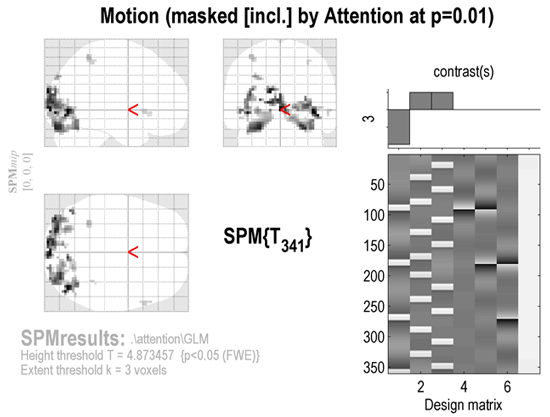
\epsfig{file=ppi/motion-attnmask,width=85mm}
\caption{\em Statistical parametric map for the \texttt{Motion} contrast inclusively masked by the Attention contrast}
\label{ppi_fig7}
\end{figure}
\end{enumerate}

\section{GLM analysis - Extracting VOIs}

\begin{enumerate}
\item First select the \texttt{Motion} contrast, but do not include masking. Use a p-value adjustment of FWE with height threshold of 0.05 and a cluster threshold of 3.
\item Go to point [15 -78 -9]
\item Press \texttt{eigenvariate}
\item Name of region [V2]
\item Adjust data for [effects of interest]
\item VOI definition [sphere]
\item VOI radius(mm) [6]
\end{enumerate}
This saves the extracted VOI data in the file \texttt{VOI\_V2\_1.mat} in the working directory, and displays Figure 1.8, below. The left side shows the location on a standard brain. The right side shows the first eigenvariate of the extracted BOLD signal.

\begin{figure}[!ht]
\centering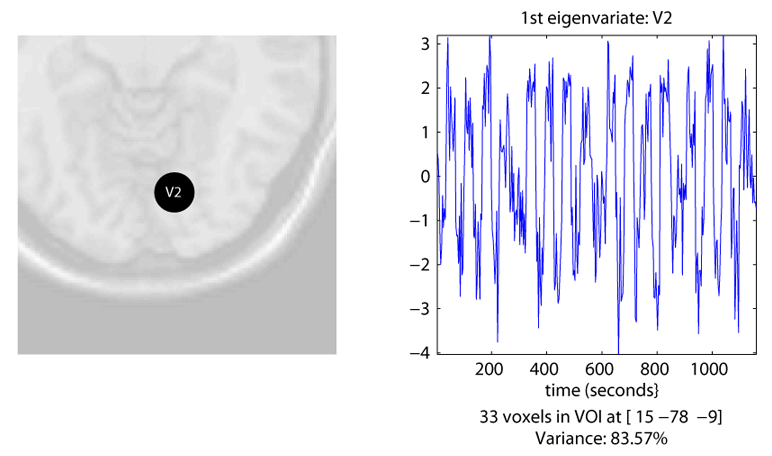
\epsfig{file=ppi/v2-eigenvariate,width=85mm}
\caption{\em First eigenvariate of the extracted BOLD signal in V2}
\label{ppi_fig8}
\end{figure}

\section{PPI analysis - Create PPI variable}
\begin{enumerate}
\item Press the \textsc{PPIs} button, and select the previous \texttt{SPM.mat} file in the \texttt{GLM} directory.
\item Analysis type ? [psychophysiologic interaction]
\item Select \texttt{VOI\_V2\_1.mat}
\item Include Fixation [No]
\item Include Stationary [No]
\item Include No-Attention [Yes], contrast weight [-1]
\item Include Attention [Yes], contrast weight [1]
\item Name of PPI [ V2x(Att-NoAtt) ]
\end{enumerate}
After a few seconds the PPI will be calculated and a graphical window will appear, see below. A file \texttt{PPI\_V2x(Att-NoAtt).mat} will be created in the current working directory. It contains the variable \texttt{PPI.ppi} (the interaction term), \texttt{PPI.Y} (the original ROI eigenvariate) and \texttt{PPI.P} (the \texttt{Attention - No Attention} task vector). You will use these vectors in setting up your psychophysiologic interaction GLM analysis. See \texttt{spm\_peb\_ppi} for a full description of the \texttt{PPI} data structure. 

\begin{figure}[!ht]
\centering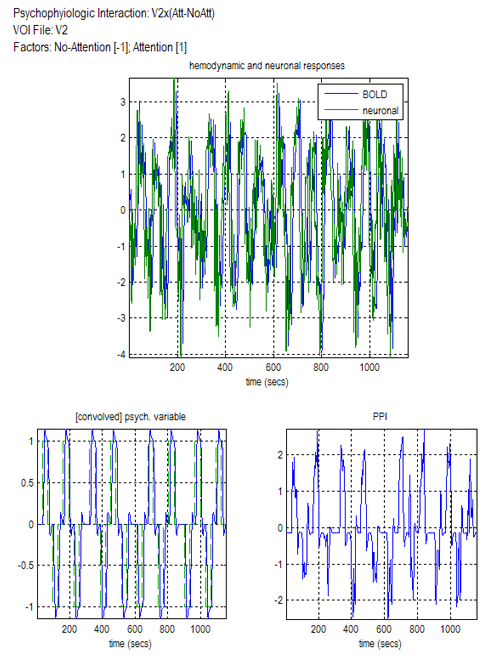
\epsfig{file=ppi/ppi-setup,width=85mm}
\caption{\em PPI output graphics}
\label{ppi_fig9}
\end{figure}

\subsection{PPI GLM analysis - Design setup and estimation}

\begin{enumerate}
\item Copy the file \texttt{PPI\_V2x(Att-NoAtt)} \textsc{Mat}-file to the \texttt{PPI} directory that you created at the start of this exercise.
\item Create a new directory and copy the file \texttt{PPI\_V2x(Att-NoAtt).mat} to this directory.
\item \texttt{cd} (change directory) to the new directory.
\item At the \matlab\ prompt type
\begin{verbatim}
>> load PPI_V2x(Att-NoAtt)
>> whos
\end{verbatim}
\item From the Tasks menu at the top of the Graphics window select Batch
\item Select \textsc{``New Stats''} from the Options box, then add jobs \textsc{New ``fMRI model specification''}, \textsc{New ``Model estimation''}, and \textsc{New ``Contrast Manager''}, and Expand All.
\item Directory: Choose the \texttt{PPI} directory
\item Units for design [scans]
\item Interscan interval [3.22]
\item Add a \textsc{New ``Subject/Session''} under \textsc{Data \& Design}
\item Click \textsc{Scans} and choose all the functional scans \texttt{snffM00587\_00xx.img}. There should be 360 \texttt{*.img} files.
\item Click \textsc{Regressors}, add 3 regressors and Expand All
\item Regressor 1: Name: \texttt{PPI-interaction}, Value: \texttt{PPI.ppi}
\item Regressor 2: Name: \texttt{V2-BOLD}, Value: \texttt{PPI.Y}
\item Regressor 3: Name: \texttt{Psych\_Att-NoAtt}, Value: \texttt{PPI.P}
\item High Pass Filter [192]
\item \textsc{Model estimation} $\rightarrow$ \textsc{Select \texttt{SPM.mat}} $\rightarrow$ \textsc{Output from ``fMRI model specification''}
\item \textsc{Contrast Manager} $\rightarrow$ \textsc{Select \texttt{SPM.mat}} $\rightarrow$ \textsc{Output from ``Model estimation''} 
\item \textsc{Contrast Manager} $\rightarrow$ \textsc{Contrast sessions} $\rightarrow$ \textsc{New ``T-contrast''}. Double click \textsc{T-contrast} to expand.
\item T-contrast: Name: \texttt{PPI-Interaction}
\item T-contrast vector: \texttt{1 0 0 0}
\item Save the batch file.
\item Run
\end{enumerate}
The design matrix is shown below, Figure 1.10.

\begin{figure}[ht]
\centering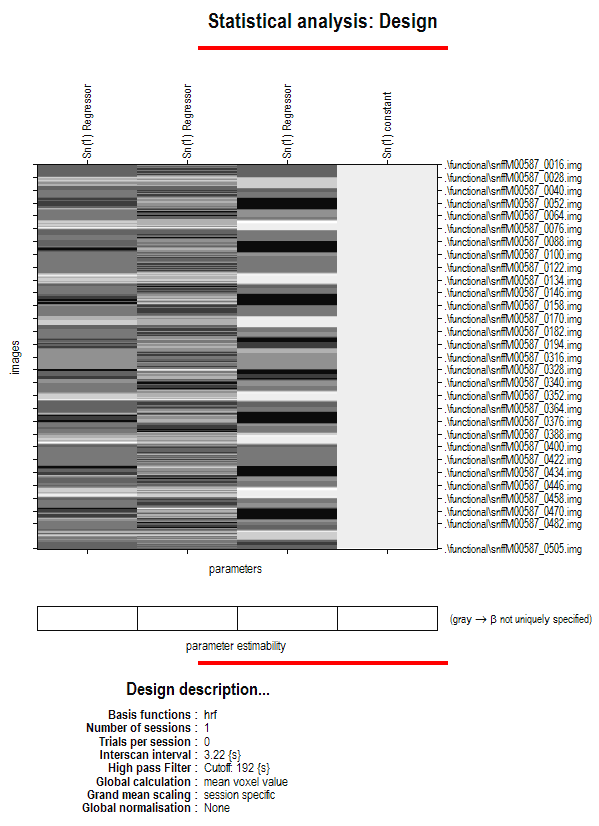
\epsfig{file=ppi/ppi-design-matrix,width=85mm}
\caption{\em Design matrix of the PPI analysis}
\label{ppi_fig10}
\end{figure}

\subsection{PPI analysis - Results}

\begin{enumerate}
\item Press the \textsc{Results} button and select the \texttt{SPM.mat} file in the PPI directory.
\item Choose the \texttt{PPI-Interaction} contrast
\item Mask with other contrasts [No]
\item Title for comparison [PPI-Interaction]
\item p value adjustment to control [None]
\item threshold {T or p value} [0.01]
\item \& extent threshold {voxels} [10]
\item You should see an SPM that looks the same as the one shown below in the top part of Figure 1.11. The resulting SPM shows areas showing differential connectivity to V2 due to the effect of attention vs. no attention conditions. The effect in this subject is weak.
\end{enumerate}

\begin{figure}[!ht]
\centering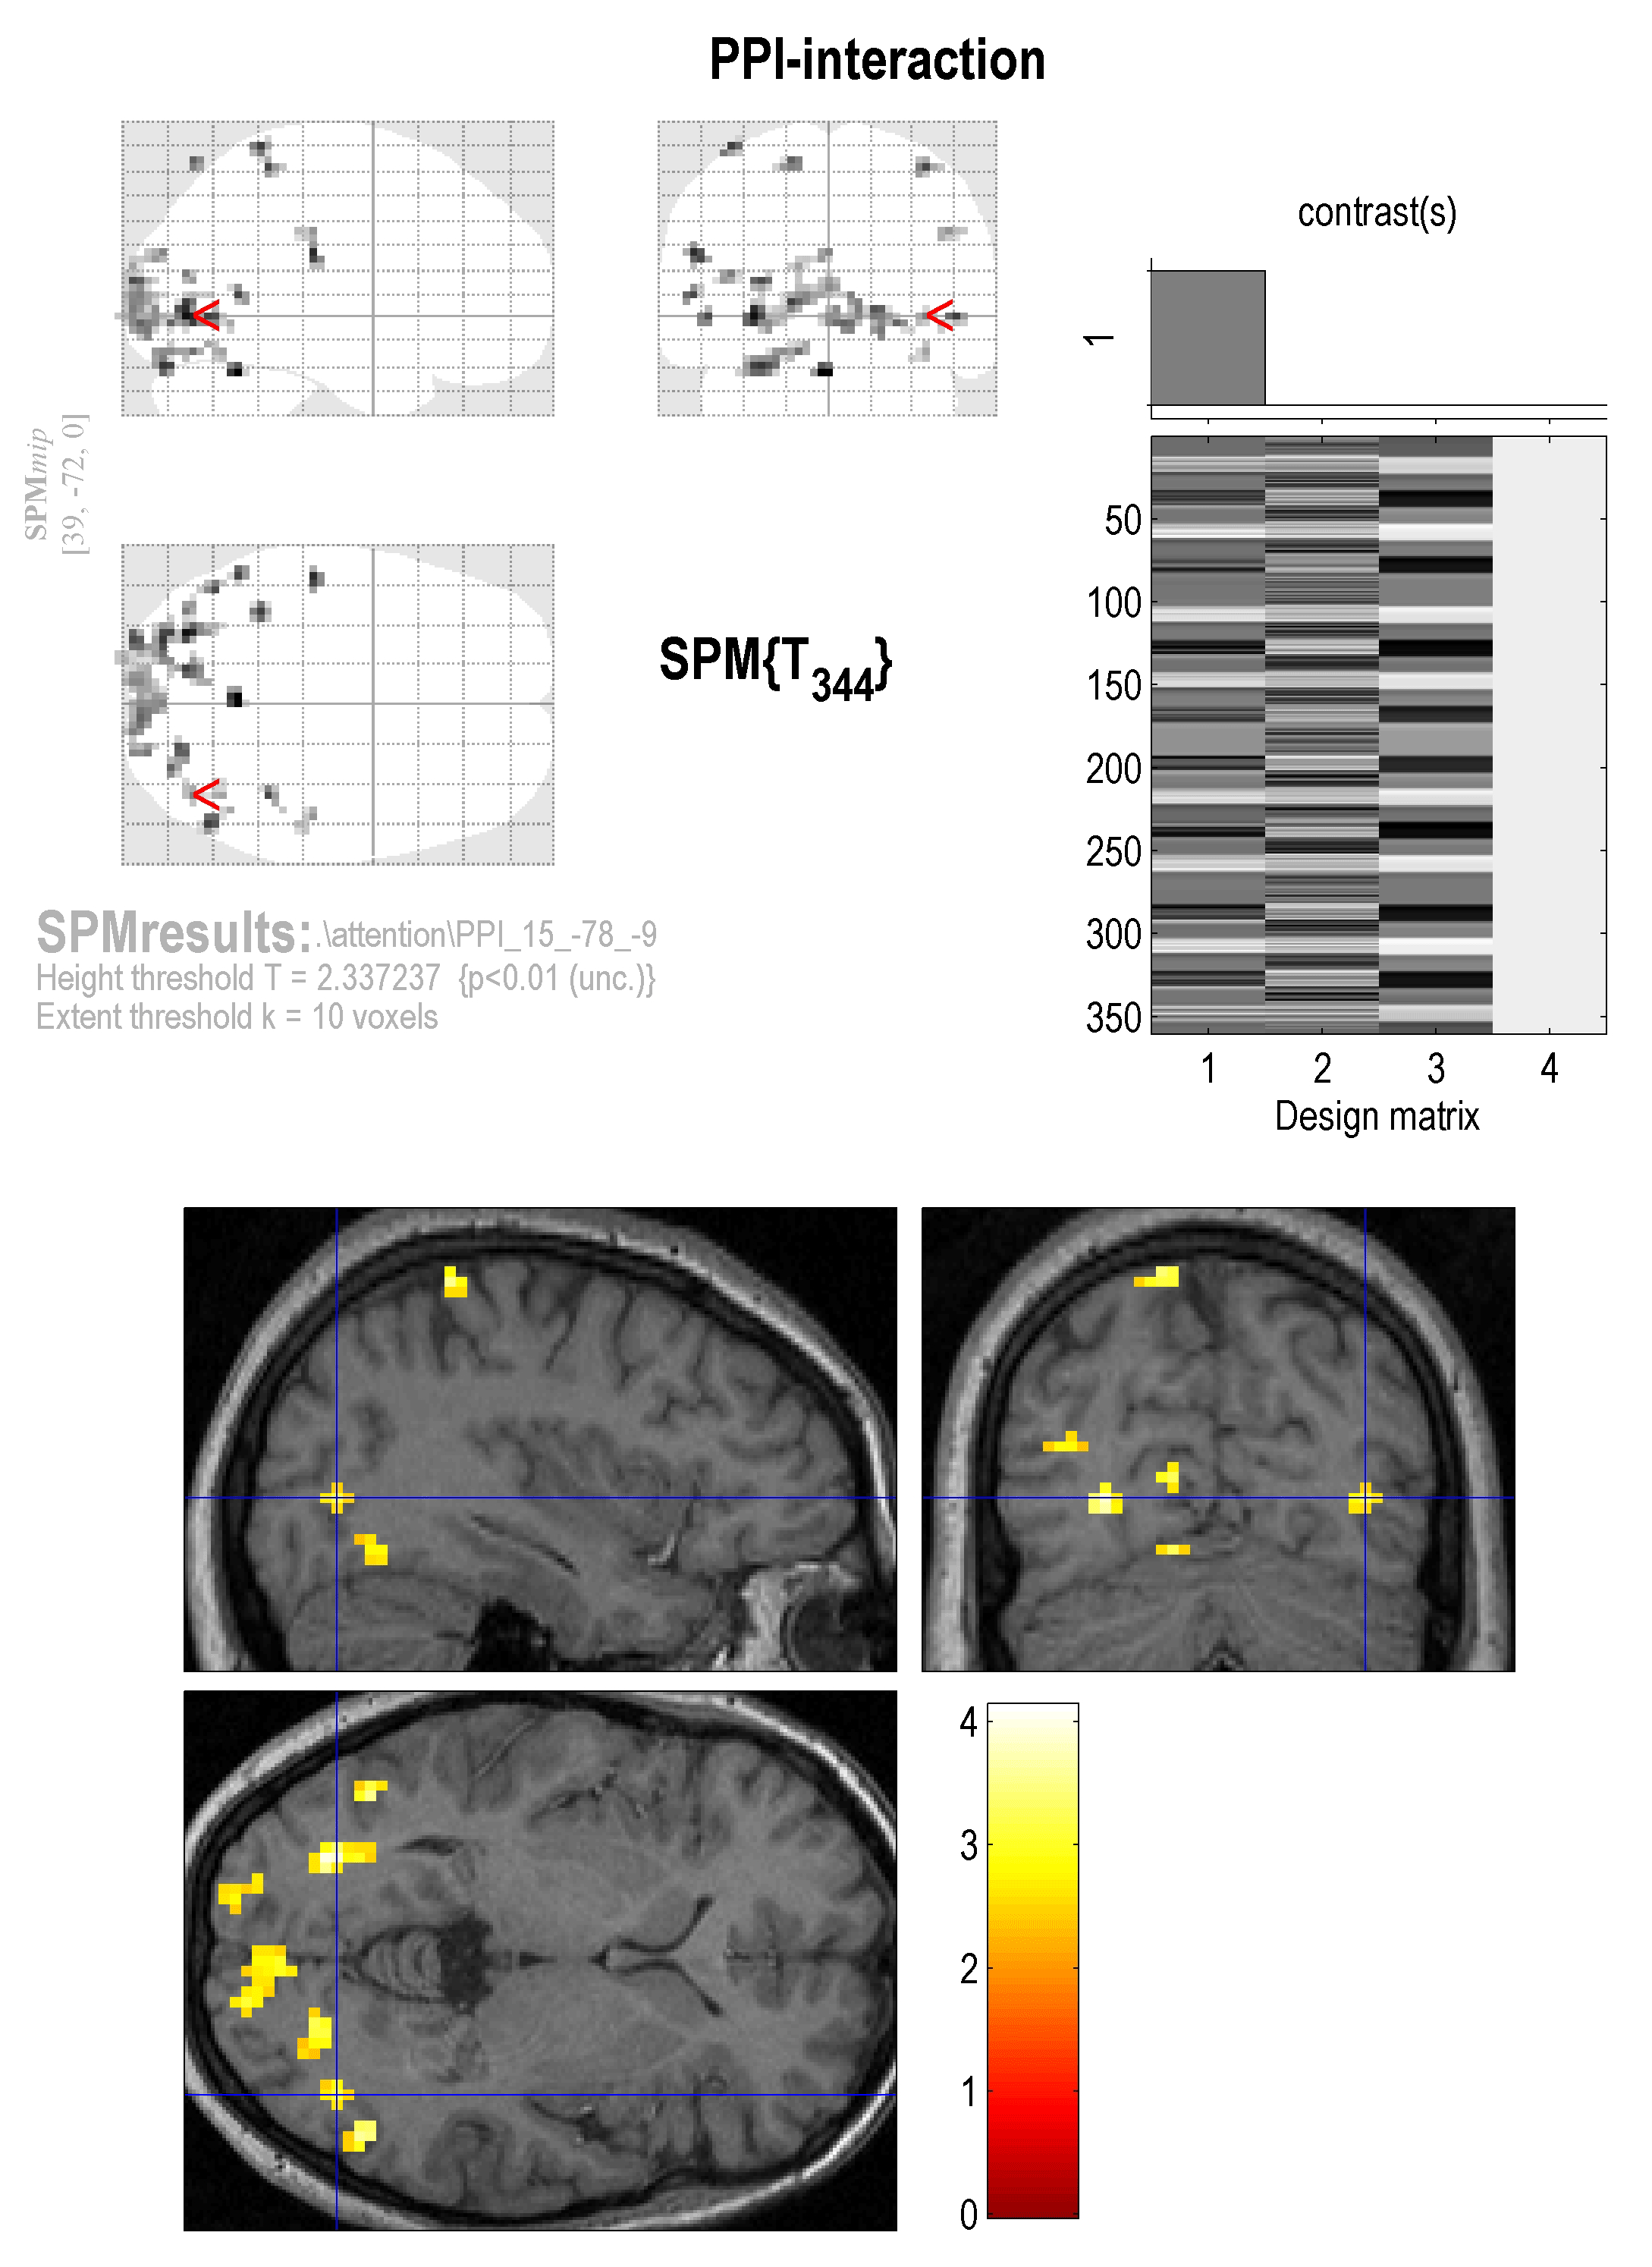
\epsfig{file=ppi/ppi-contrast,width=100mm}
\caption{\em PPI results}
\label{ppi_fig11}
\end{figure}

\subsection{PPI analysis - Plotting}

\begin{enumerate}
\item One region showing the psychophysiologic interaction is the V5region , which is located at [39~-72~0] in this subject. Move the cursor to this point to view the area of activation, as shown below, in the bottom half of Figure 1.11.

\item In order to plot the PPI graph showing the effect of attention, you need to extract a VOI from the V5 region. To do this, you will return to the original GLM analysis.
\item Click Results, then select the GLM analysis \texttt{SPM.mat} file
\item Mask with other contrasts [No]
\item Title for comparison [Motion]
\item p value adjustment to control [None]
\item threshold {T or p value} [0.001]
\item \& extent threshold {voxels} [3]
\item Go to point [39- 72 0]
\item Press eigenvariate
\item Name of region [V5]
\item Adjust data for [effects of interest]
\item VOI definition [sphere]
\item VOI radius(mm) [6]
\item Now you will create 4 PPIs (Follow the steps under section 1.4, Create PPI Variable, above). By using the PPI software machinery to create the interaction vectors, rather than just multiplying the extracted V2 and V5 eigenvariates by the behavioral vectors, the PPI vectors will be formed properly.

\begin{enumerate}
\item \texttt{V2xNoAttention} (Use the V2 VOI and include \texttt{No-Attention} with a contrast weight of 1, do not include \texttt{Stationary}, \texttt{Attention})
\item \texttt{V2xAttention} (Use the V2 VOI and include \texttt{Attention} with a contrast weight of 1, do not include \texttt{Stationary}, \texttt{No-Attention})
\item \texttt{V5xNoAttention} (Use the V5 VOI and include \texttt{No-Attention} with a contrast weight of 1, do not include \texttt{Stationary}, \texttt{Attention})
\item \texttt{V5xAttention} (Use the V5 VOI and include \texttt{Attention} with a contrast weight of 1, do not include \texttt{Stationary}, \texttt{No-Attention})
\end{enumerate}
\item Load the PPIs you just created with the following commands at the \matlab\ prompt:
\begin{verbatim}
>> v2noatt = load('PPI_V2xNoAttention');
>> v2att   = load('PPI_V2xAttention.mat');
>> v5noatt = load('PPI_V5xNoAttention.mat');
>> v5att   = load('PPI_V5xAttention.mat');
\end{verbatim}
\item Plot the PPI datapoints with the following commands at the \matlab\ prompt:
\begin{verbatim}
>> figure
>> plot(v2noatt.PPI.ppi,v5noatt.PPI.ppi,'k.');
>> hold on
>> plot(v2att.PPI.ppi,v5att.PPI.ppi,'r.');
\end{verbatim}
\item To plot the best fit lines type the following first for \texttt{NoAttention}
\begin{verbatim}
>> x  = v2noatt.PPI.ppi(:);
>> x  = [x, ones(size(x))];
>> y  = v5noatt.PPI.ppi(:);
>> B  = x\y;
>> y1 = B(1)*x(:,1)+B(2);
>> plot(x(:,1),y1,'k-');
\end{verbatim}
\item Then for \texttt{Attention}
\begin{verbatim}
>> x = v2att.PPI.ppi(:);
>> x = [x, ones(size(x))];
>> y = v5att.PPI.ppi(:);
>> B = x\y;
>> y1 = B(1)*x(:,1)+B(2);
>> plot(x(:,1),y1,'r-');
>> legend('No Attention','Attention')
>> xlabel('V2 activity')
>> ylabel('V5 response')
>> title('Psychophysiologic Interaction')
\end{verbatim}
\end{enumerate}

\begin{figure}[!ht]
\centering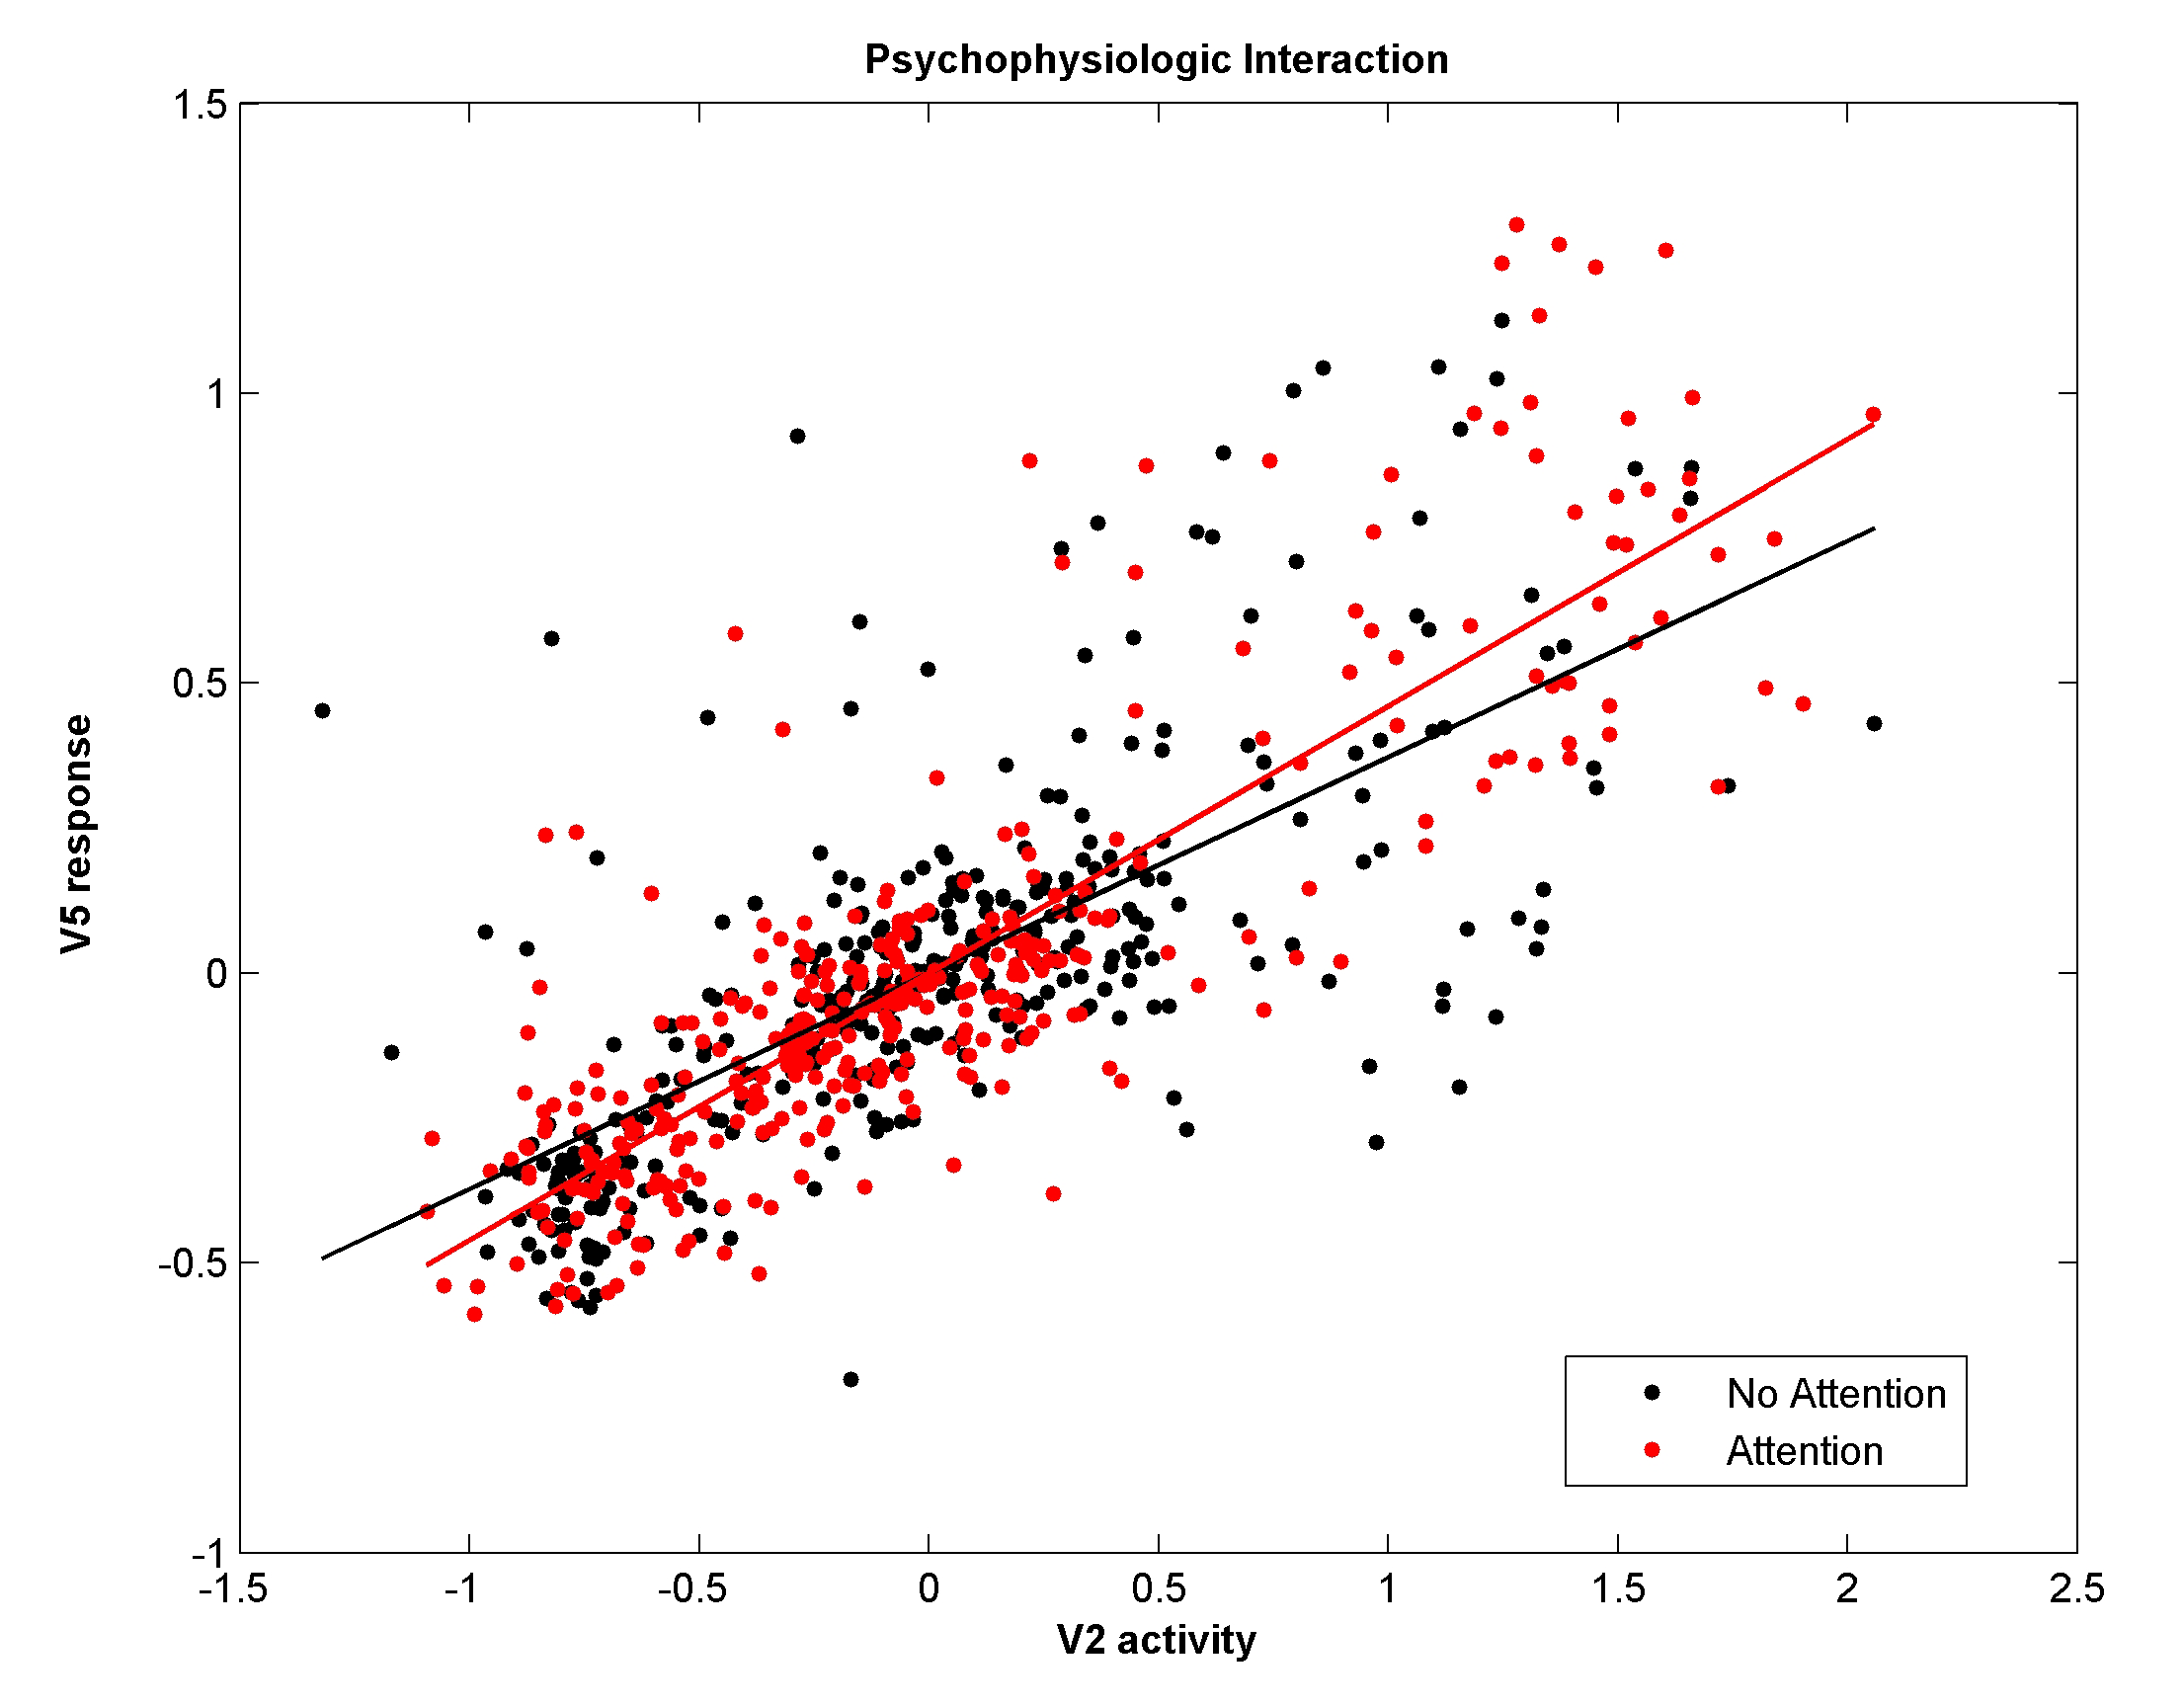
\epsfig{file=ppi/ppi-plot,width=110mm}
\caption{\em }
\label{ppi_fig12}
\end{figure}